\chapter{Các công trình liên quan}
\label{Chapter2}

Bài toán sinh cử chỉ là cũng tương tự như các bài toán khác đều đã nghiên cứu và phát triển song hành cùng các phương pháp học máy truyền thống cũng như các phương pháp học sâu hiện đại ngày nay, gồm các nhóm phương pháp dựa trên luật và các phương pháp dựa trên dữ liệu. 

\section{Mối quan hệ giữa cử chỉ và lời nói}

Cử chỉ được chia thành 6 nhóm chính theo ngôn ngữ  học \cite{ekman1969repertoire}, \cite{sebeok2011advances} cử chỉ thích nghi (adaptors), cử chỉ biểu tượng (emblems), cử chỉ chỉ định (deictics), cử chỉ biểu trưng (iconics), cử chỉ ẩn dụ (metaphorics) và cử chỉ nhấn mạnh (beat).

 Trong đó, cử chỉ nhấn mạnh không liên quan trực tiếp đến ngữ nghĩa lời nói \cite{kipp2005gesture} nhưng rất quan trọng để tạo sự hài hòa về nhịp điệu giữa lời nói và cử chỉ  \cite{sebeok2011advances} . Tuy nhiên, lời nói và cử chỉ nhấn mạnh không đồng bộ hoàn toàn về mặt nhịp điệu \cite{mcclave1994gestural}, nên việc học mối liên hệ thời gian giữa chúng gặp khó khăn \cite{bhattacharya2021speech2affectivegestures}, \cite{kucherenko2020gesticulator}, \cite{yoon2020speech}.

Cử chỉ liên quan đến các cấp độ khác nhau của thông tin lời nói \cite{sebeok2011advances}. Ví dụ, cử chỉ biểu tượng như cầm ngược cái ngón cái thường đi kèm với ngữ nghĩa cấp cao như tốt hay tuyệt vời, trong khi cử chỉ nhấn mạnh thường xuất hiện cùng với sự nhấn mạnh âm thanh cấp thấp. Nhiều nghiên cứu trước đây chỉ sử dụng các đặc trưng được trích xuất từ lớp cuối cùng của bộ mã hóa âm thanh để tổng hợp cử chỉ \cite{alexanderson2020style},  \cite{bhattacharya2021speech2affectivegestures}, \cite{kucherenko2021large}, \cite{qian2021speech},  \cite{yoon2022genea}. Tuy nhiên, cách thiết lập này có thể khuyến khích bộ mã hóa trộn lẫn thông tin lời nói ở nhiều cấp độ khác nhau vào cùng một đặc trưng, gây ra sự mơ hồ và tăng độ khó khăn trong việc khai thác các dấu hiệu nhịp điệu và ngữ nghĩa rõ ràng.

%Trong bài báo này, chúng tôi tập trung vào việc tạo ra cử chỉ trên đi kèm lời nói có thể đồng hành với một loạt các nội dung lời nói rộng - từ một câu đến bài phát biểu công khai, nhằm đạt được kết quả thuyết phục cả về nhịp điệu và ngữ nghĩa. Quan sát đầu tiên của chúng tôi là cử chỉ có thể được coi là một dạng nhảy đặc biệt dưới nhịp điệu thay đổi. Chúng tôi phát triển một khuôn khổ chuẩn hóa và tạo ra nhịp điệu để đối phó với thách thức tạo ra cử chỉ đồng bộ với lời nói, phân đoạn lời nói thành các đoạn ngắn tại các nhịp âm thanh, chuẩn hóa các đoạn này thành các khối chuẩn có cùng độ dài, tạo ra cử chỉ cho mỗi khối và căn chỉnh chuyển động được tạo ra với nhịp điệu của lời nói. Khuôn khổ này, được lấy cảm hứng một phần từ các nghiên cứu gần đây về tạo múa \cite{aristidou2022rhythm}, cung cấp cho mô hình cử chỉ một gợi ý rõ ràng về nhịp điệu, cho phép mô hình học hiệu quả mẫu cử chỉ nhấn mạnh trong một khối nhịp điệu. 
%Cả đánh giá định lượng với một chỉ số nhịp điệu mới và đánh giá chất lượng với nghiên cứu người dùng đều cho thấy cử chỉ được tạo ra bởi quy trình này thể hiện sự đồng bộ tự nhiên với lời nói.

Như được chỉ ra trong các tài liệu ngôn ngữ học \cite{kipp2005gesture} \cite{neff2008gesture} \cite{webb1997linguistic},
cử chỉ được sử dụng trong cuộc hội thoại hàng ngày có thể được chia thành một số lượng hạn chế các đơn vị ngữ nghĩa với các biến thể chuyển động khác nhau. Chúng tôi giả định rằng các đơn vị ngữ nghĩa này, thường được gọi là từ ngữ, liên quan đến các đặc trưng cấp cao của âm thanh lời nói, trong khi các biến thể chuyển động được xác định bởi các đặc trưng âm thanh cấp thấp. Do đó, chúng tôi tách rời các đặc trưng cấp cao và cấp thấp từ các lớp khác nhau của bộ mã hóa âm thanh và học các ánh xạ giữa chúng và các từ ngữ cử chỉ và các biến thể chuyển động, tương ứng. Các thử nghiệm chứng minh cơ chế này thành công trong việc tách rời các đặc trưng ở nhiều cấp độ của cả lời nói và chuyển động và tổng hợp các cử chỉ phù hợp về mặt ngữ nghĩa và có phong cách.

\section{Các phương pháp cho bài toán sinh cử chỉ}

\subsection{Phương pháp dựa trên luật}

Các phương pháp dựa trên luật thường ánh xạ (mappings) từng âm thanh với từng đơn vị cử chỉ \cite{huang2012robot}. Và luật được tạo thủ công. Phương pháp dựa trên luật thì chúng ta có thể dễ dàng điều khiển kết quả của mô hình và có khả năng giải thích tốt kết quả dự đoán của mô hình.
Tuy nhiên chi phí để tạo thủ công là không khả thi để xây dựng cho các ứng dụng phức tạp.

\subsection{Phương pháp dựa trên thống kê}

Tương tự như phương pháp dựa trên luật, phương pháp dựa trên dữ liệu cũng ánh xạ các đặc trưng của âm thanh tương ứng với cử chỉ nhưng thay vì làm thủ công thì được sử dụng học một cách tự động dựa trên dữ liệu.
Trong đó có hai phương pháp chính là phương pháp thống kê và phương pháp dựa trên dữ liệu.


\subsubsection{Phương pháp thống kê}

Phương pháp thống kê sử dụng phân phối xác xuất để tìm sự tương đồng giữa các đặc trưng âm thanh và cử chỉ \cite{levine2010gesture}. Tác giả \cite{neff2008gesture} xây dựng mô hình để học từng phong cách của từng người nói.

\subsubsection{Phương pháp học sâu}

\setcounter{figure}{3}
\begin{figure}
	\centering
	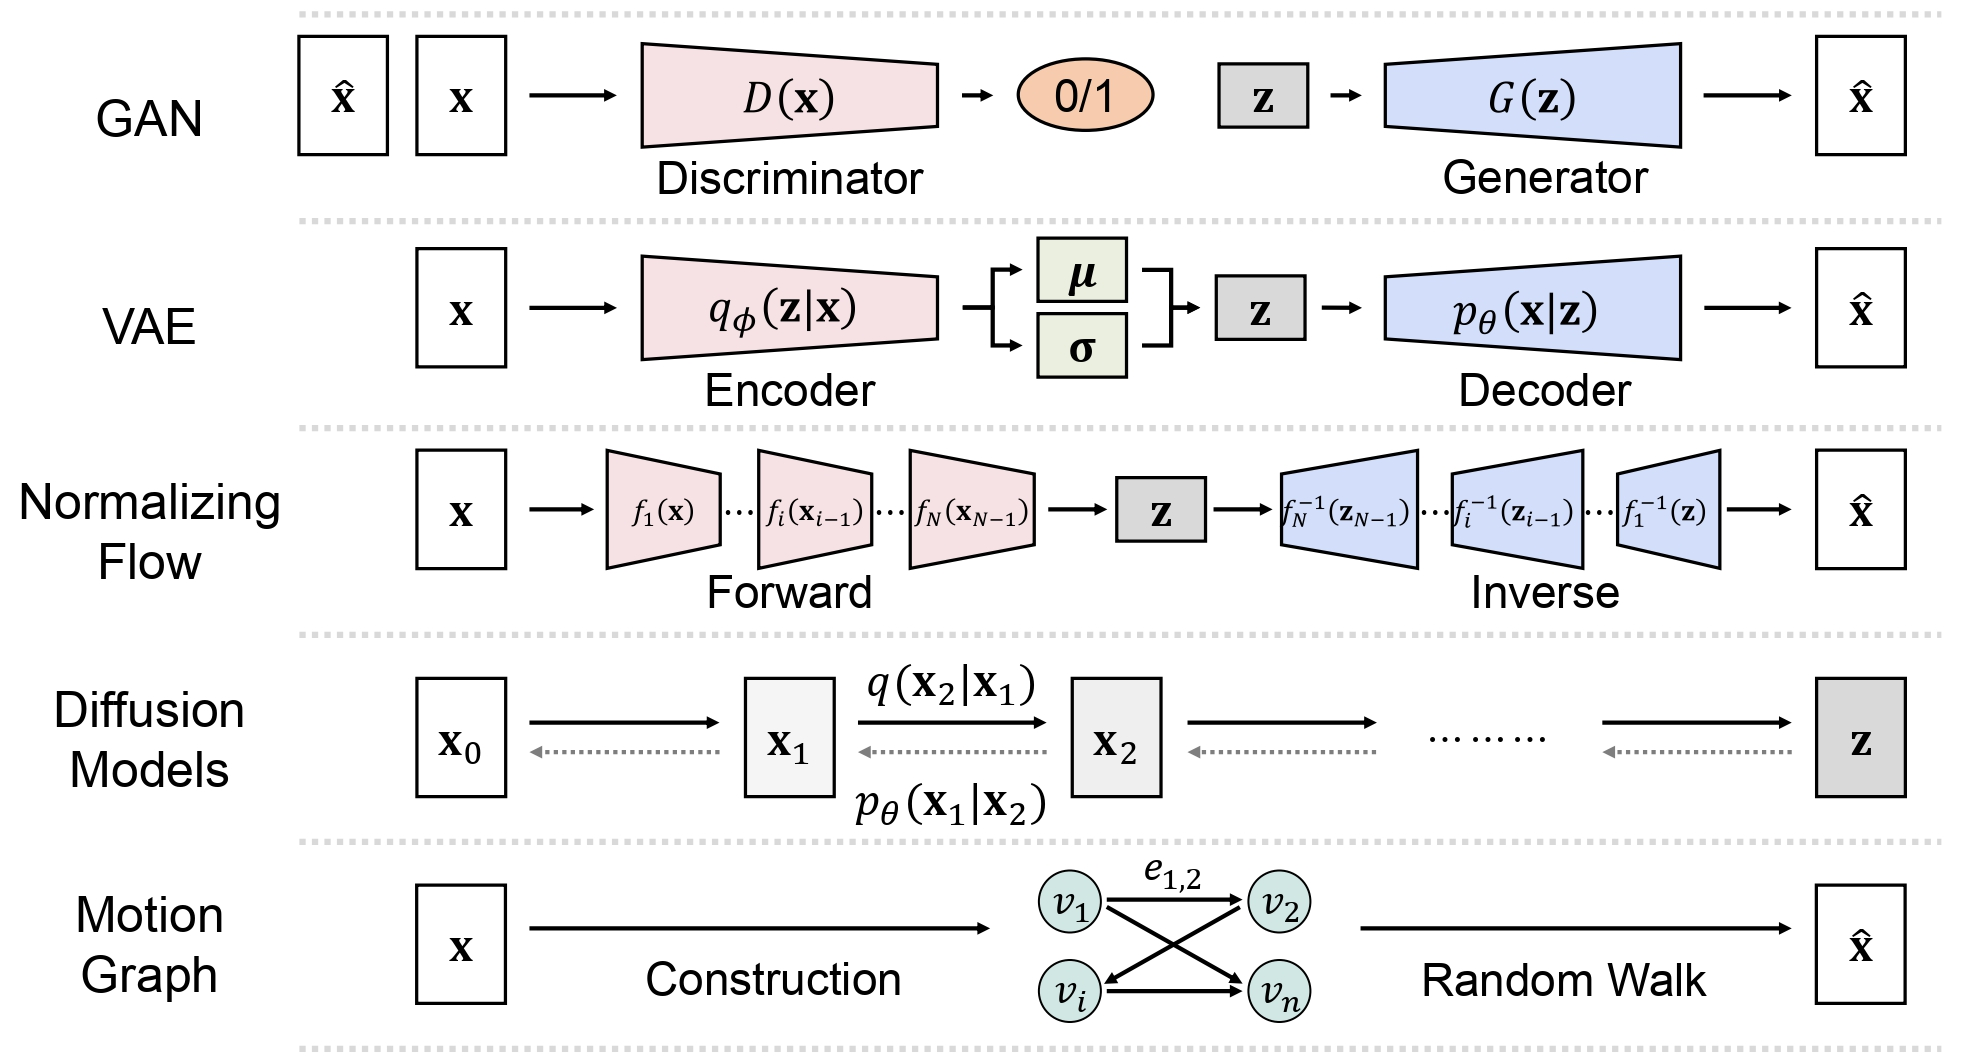
\includegraphics[width=0.8\textwidth]{Survey.jpg}
	\caption{Tổng quan về các mô hình tạo sinh khác nhau.}
	\label{fig:generative-models}
\end{figure}

Phương pháp học sâu sử dụng mạng nơ-ron (neural) thông qua nhiều lớp ẩn để học một cách tự động các phối xác xuất giữa cử chỉ và âm thanh.

Mô hình được kết hợp với văn bản đầu vào được gắn thẻ với chủ đề, trọng tâm câu và thành ngữ để tạo ra các kịch bản cử chỉ, sau đó được ánh xạ sang một chuỗi các cử chỉ được chọn từ một từ điển hoạt họa. \cite{chiu2015predicting} huấn luyện một mô hình phân loại thần kinh để chọn một đơn vị cử chỉ phù hợp dựa trên đầu vào lời nói. Nghiên cứu gần đây đã bắt đầu tận dụng học sâu và huấn luyện các mô hình kết thúc đến cuối sử dụng dữ liệu cử chỉ thô trực tiếp, giải phóng các nỗ lực thủ công trong thiết kế từ điển cử chỉ và các quy tắc ánh xạ. Cử chỉ có thể được tổng hợp bằng các mô hình xác định như perceptron đa tầng (MLP) \cite{kucherenko2020gesticulator}, recurrent neural networks \cite{bhattacharya2021speech2affectivegestures}, \cite{liu2022learning}, \cite{hasegawa2018evaluation}, \cite{yoon2020speech}, convolutional networks \cite{habibie2021learning} và transformer \cite{bhattacharya2021text2gestures} và các mô hình như normalizing flow \cite{alexanderson2020style}, WGAN \cite{wu2021probabilistic}.
%phương pháp học code  \cite{xu2022freeform}.

%\section{Mô hình diffusion}



Với đặc điểm dữ liệu là giá trị của các góc quay, các toạ độ của điểm khớp, nên cần độ chi tiết cao để tạo ra sự chân thực trong các chuyển động của nhân vật. Ngoài ra dữ liệu sẽ thiếu và rất ít dữ liệu trong các trường hợp cực trị của tham số.
Nên chúng tôi sử dụng mô hình Diffusion, với đặc điểm là có thể học được độ chi tiết cao hơn và có thể phủ được dữ liệu trong các trường hợp cực trị của tham số và độ phủ về mật độ dữ liệu thấp.

%\textbf{Bảng so sánh các phương pháp}
%
%\begin{table}[ht]
%	\centering
%	\begin{tabular}{|l|l|l|l|l|l|}
%		\hline
%		\textbf{Phương pháp} & \textbf{Loại mô hình} & \textbf{Đặc điểm nổi bật} & \textbf{Ưu điểm} & \textbf{Hạn chế} & \textbf{Tài liệu tham khảo} \\ \hline
%		VAE  & Autoencoder & Biểu diễn dữ liệu trong không gian tiềm ẩn & Tạo đặc trưng ẩn & Khó kiểm soát đầu ra & \cite{kingma2013auto} \\ \hline
%		VQ-VAE & Autoencoder (cải tiến) & Dùng codebook cho không gian tiềm ẩn & Biểu diễn chi tiết hơn & Phức tạp hơn & \cite{van2017neural} \\ \hline
%		RNN & Mạng hồi tiếp & Xử lý chuỗi dữ liệu & Tốt cho dữ liệu tuần tự & Khó huấn luyện & \cite{bhattacharya2021speech2affectivegestures} \\ \hline
%		Transformer & Mạng chú ý & Tạo cử chỉ qua cơ chế chú ý & Hiệu quả với dữ liệu dài & Yêu cầu nhiều tài nguyên & \cite{bhattacharya2021text2gestures} \\ \hline
%		WGAN & GAN & Học phân phối dữ liệu đối kháng & Tạo sự đa dạng & Khó huấn luyện & \cite{wu2021probabilistic} \\ \hline
%		Normalizing Flow & Mô hình xác suất & Học phân phối phức tạp & Hữu ích với dữ liệu phức tạp & Cần tài nguyên tính toán lớn & \cite{alexanderson2020style} \\ \hline
%		Diffusion Models & Mô hình sinh dữ liệu & Chi tiết cao, xử lý dữ liệu thiếu & Tạo cử chỉ chi tiết & Thời gian huấn luyện lâu & \cite{xu2022freeform} \\ \hline
%	\end{tabular}
%	\caption{So sánh các phương pháp sinh cử chỉ}
%\end{table}

%
%Với các phương pháp dựa trên luật hoặc thống kê, mô hình có thể đạt được kết quả tốt và dễ dàng điều khiển, tuy nhiên để có thể ứng dụng vào thực tế. Đòi hỏi mô hình cần học từ hàng triệu điểm dữ liệu. Điều này khiến việc dùng các mô hình học truyền thống kém khả thi.
%
%Mô hình sinh cử chỉ của chúng tôi dựa trên neural network, cụ thể là mô hình VQ-VAE.
%Mô hình VQ-VAE \cite{van2017neural}, hay còn được gọi là Vector Quantize Variational Autoencoder là mô hình cải tiến của VAE \cite{kingma2013auto} (Variational Autoencoder). 
%Mô hình VAE biểu diễn toàn bộ dữ liệu trên không gian tiềm ẩn (latent space) và từ không gian tiềm ẩn giải mã (decoder) ngược trở lại dữ liệu ban đầu với mục tiêu là học được các tham số của phân phối chuẩn mà vẫn giữ được nhiều nhất các đặc trưng của dữ liệu.
%Trong khi đó, cải tiến của mô hình VQ-VAE là biểu diễn toàn bộ không gian tiềm ẩn thành nhiều vùng khác nhau với mỗi vùng là một code đại diện, tập hợp các code được gọi là codebook. Việc huấn luyện để biểu diễn các dữ liệu thành một đại diện code trong nhiều vùng giúp mô hình có thể biểu diễn tốt hơn so với VAE chỉ biêu diễn dữ liệu thành các phân phối chuẩn.

% Hầu hết các nghiên cứu hiện tại về việc dự đoán liên kết của đồ thị tri thức đều liên quan đến các phương pháp tiếp cận tập trung vào khái niệm nhúng một đồ thị đã cho trong một không gian vectơ có số chiều thấp. Ngược lại với các tiếp cận này là một phương pháp đựa trên luật được nghiên cứu trong \cite{burl}. Thuật toán cốt lõi của nó dựa trên lấy mẫu một luật bất kỳ, sau đó khái quát  thành các quy tắc Horn\cite{wiki:Horn}. Tiếp đó dùng thống kê để tính độ tin cậy của các luật được khái quát. Khi dự đoán một liên kết mới (cạnh mới) của đồ thị chúng ta dự đoán một đỉnh có cạnh nối với một quan hệ cụ thể (label) với đỉnh còn lại hay không. Cũng đã có rất nhiều phương pháp được nghiên cứu, đề xuất để học các các luật trong đồ thị chẳng hạn như trong  RuDiK\cite{ortona2018robust}, AMIE\cite{galarraga2015fast}, RuleN\cite{meilicke2018fine}. 
% Như đã nói trong phần trước có hai cách tiếp cận chính cho bài toán này một là tối ưu hóa hàm mục tiêu. Tìm ra một bộ quy tắc nhỏ bao gồm phần lớn các ví dụ là đúng và ít sai sót nhất có thể như được ngiên cứu trong RuDiK\cite{ortona2018robust}. Còn cách tiếp cận còn lại cũng là cách tiếp cận mà chúng tôi chọn nghiên cứu là cố gắng tìm hiểu mọi quy tắc khả thi có thể sau đó tạo xếp hạng \(k\) ứng viên tiềm năng với một độ tin cậy nhất định được đo trên tập huấn luyện.

% Phương pháp đựa trên luật của chúng tôi phần lớn dựa vào phương pháp Anytime Bottom-Up Rule Learning for Knowledge Graph Completion \cite{meilicke2019anytime} mà sau đây chúng tôi gọi là \textbf{AnyBURL}. Như tên của phương pháp này phương pháp chủ yếu chú trọng vào vấn đề hoàn thành đồ thị, điền những phần còn thiếu vào đồ thị. Vấn đề tồn đọng lại ở mô hình này khi có một cạnh mới hay một tri thức mới được thêm vào đồ thị sẽ phải đào tạo lại toàn bộ mô hình. Chúng tôi giải quyết vẫn đề này theo hai ch iến lược offline-to-online tức là khi thêm vào đồ thị tập hợp các cạnh thì mới thực hiện lại quá trình đào tạo lại một phần của đồ thị và chiến lược thứ 2 là online-to-online  khi thêm một cạnh mới sẽ thực hiện đào tạo lại ngay một phần có liên quan tới cạnh vừa thêm vào.

% % GAT
% Trong nhánh các phương pháp về học sâu, rất nhiều kỹ thuật học sâu thành công trong xử lý ảnh và xử lý ngôn ngữ tự nhiên được áp dụng vào đồ thị tri thức như : Mạng Neural Tích Chập (Convolution Neural Network - CNN \cite{lecun1999object}), Mạng Neural Hồi Quy (Recurrent Neural Network\cite{hopfield2007hopfield}), và gần đây như Transformer (\cite{yang2019xlnet}), Mạng Neural Bao Bọc (Capsule Neural Network - CapsNet \cite{sabour2017dynamic}). Bên cạnh đó các nghiên cứu còn sử dụng một số kỹ thuật khác như Random Walks, các mô hình dựa trên cấu trúc phân cấp, .. Ưu điểm chung của nhóm các phương pháp học sâu trên đồ thị tri thức đó là tự động rút trích các đặc trưng và có thể khái quát hóa cấu trúc phức tạp của đồ thị dựa trên một lượng lớn dữ liệu huấn luyện. Tuy nhiên, một số phương pháp chỉ chủ yếu tập trung vào cấu trúc dạng lưới mà không giữ được đặc trưng không gian của đồ thị tri thức. 
% Cơ chế chú ý hay lớp chú ý đa đỉnh (multi-head attention layer) đã được áp dụng vào đồ thị bằng mô hình Mạng Đồ Thị Chú Ý (Graph Attention Network - GAT \cite{velivckovic2017graph}) giúp tổng hợp thông tin của một thực thể dựa vào trọng số chú ý của thực thể gốc đối với các thực thể lân cận. Tuy nhiên, mô hình đồ thị chú ý lại thiếu thông tin của vector nhúng quan hệ cũng như các vector nhúng lân cân của một thực thể gốc, một phần rất quan trọng giúp thể hiện vai trò của từng thực thể. Vấn đề đó đã được giải quyết trong báo cáo Learning Attention-based Embeddings for Relation Prediction in
% Knowledge Graphs (\textbf{KBAT} \cite{nathani2019learning}), mô hình được chúng tôi chọn làm cơ sở nghiên cứu.
% Cơ chế chú ý đang là một trong những cấu trúc học sâu đạt được hiệu quả nhất hiện nay (state-of-the-art) vì nó đã được chứng minh là thay thế cho bất kỳ phương pháp tính tích chập nào \cite{cordonnier2019relationship},
% hơn nữa nó cũng nằm trong cấu trúc cơ bản để áp dụng trên các mô hình mới nhất trên ngôn ngữ tự nhiên như mô hình Megatron-LM \cite{shoeybi2019megatron}, và trên phân đoạn hình ảnh như mô hình HRNet-OCR (Hierarchical Multi-Scale Attention \cite{tao2020hierarchical}). Một số phương pháp thú vị \cite{cordonnier2020multi} đã cải tiến dựa trên cơ chế chú ý, tuy nhiên nó lại chưa được áp dụng vào đồ thị tri thức, vì vậy chúng tôi chọn nhóm phương pháp này để áp dụng các cải tiến mới nhất vào đồ thị tri thức.